% TODO
% - Bäume (26)
% - Motivation - das kann man noch deutlich besser machen. (Aber wie?)
% - evtl. Strenger Zusammenhang


\section{Graphen}
\begin{frame}{Graphen -- Wofür?}
	\begin{itemize}
		\item Straßennetze und andere Verkehrsnetze (Kürzeste Wege)
		\item Kabelnetze (Minimale Spannbäume)
		\item Rohrnetze (Maximaler Fluss)
	\end{itemize}

	\begin{block}{Zitat}
		\enquote{Egal für wie wichtig du Graphen in der Informatik hältst, sie sind mindestens doppelt so wichtig!}\\
		\emph{Ein Google-Manager über Einstellungsgespräche bei Google}
	\end{block}
\end{frame}

\subsection{Definitionen}

\begin{frame}{Graphen}
	\begin{Definition}
		Ein \textbf{gerichteter Graph} ist ein Paar $G = (V, E)$ mit einer \emph{endlichen}, \emph{nichtleeren} Menge an \textbf{Knoten} $V$ und einer Menge an \textbf{Kanten}\\
		$E \subseteq V \times V$.
	\end{Definition} \pause
	$E$ enthält also Paare (geordnet) von Elementen aus $V$. \pause
	
	\bigskip
	\begin{Definition}
		Ein \textbf{ungerichteter Graph} ist ein Paar $G = (V, E)$ mit einer \emph{endlichen}, \emph{nichtleeren} Menge an \textbf{Knoten} $V$ und einer Menge an \textbf{Kanten}\\
		$E \subseteq \set{ \{x,y\} \Mid x \in V \land y \in V }$.
	\end{Definition} \pause
	$E$ enthält also Mengen (ungeordnet) mit je ein oder zwei Elementen aus $V$!
\end{frame}

\begin{frame}{Graphen}
	\begin{block}{Hinweis}
		Häufig wählt man $V = \Z_k = \{0,1,2,...,k-1\}$\\
		
		Da $V$ immer endlich ist, muss auch $E$ endlich sein.\\
		$E = \emptyset$ ist aber erlaubt!
	\end{block}

	\pause
	\begin{Definition}
		Zwei Knoten $x$ und $y$ in einem Graphen $G$ heißen \textbf{adjazent}, wenn sie durch eine Kante verbunden sind.
	\end{Definition}
	Achtung: Im gerichteten Fall ist diese Aussage nicht symmetrisch!

	\pause
	\begin{Definition}
		Eine Kante mit identischem Start- und Endpunkt nennt man \textbf{Schlinge}.\\
		Also $(x,x) \in E$ bzw. $\{x\} \in E$\\
	\end{Definition}
\end{frame}

\begin{frame}{Beispiel}
	Wir betrachten den gerichteten Graphen $G = (V, E)$ mit $V = \{0,1,2,3,4,5\}$ und $E = \set{(0,1), (1,0), (1,2), (3,4), (4,3) ,(4,5)}$
	\bigskip

	\begin{figure}[H]
		\begin{tikzpicture}[->,>=stealth,baseline=-5mm]
		\matrix[matrix of math nodes,nodes={draw,circle,minimum size=10mm,inner sep=2pt},row sep=15mm,column sep=15mm,ampersand replacement=\&]
		{
			|(1)| 1 \& |(5)| 5 \& |(3)| 3 \\
			|(0)| 0 \& |(2)| 2 \& |(4)| 4 \\
		};
		\draw  (0) to [bend left] (1);
		\draw  (1) to [bend left] (0);
		\draw  (1) -- (2);
		
		\draw  (4) -- (5);
		\draw  (4) to [bend left] (3);
		\draw  (3) to [bend left] (4);
		\end{tikzpicture}
	\end{figure}

\end{frame}

\begin{frame}{Aufgabe: Graphen zeichnen}
	Zeichnet die Graphen $G_i = (V, E_i)$ mit $V = \Z_4$ und
	$E_1 = \{(0,1), (0,2), (0,3), (1,2), (1,3), (2,2), (2,3), (3,2)\}$\\
	$E_2 = \{\{0,1\}, \{0,2\}, \{0,3\} \}$\\
	$E_3 = \emptyset$\\
	$E_4 = V \times V$\\
	$E_5 = \{(0,1), (1,2), (1,3)\}$
\end{frame}

\begin{frame}{Lösung: Graphen Zeichnen}
	Zeichnet den Graphen $G = (V, E)$ mit
	$$V = \Z_4 \qquad E = \{(0,1), (0,2), (0,3), (1,2), (1,3), (2,2), (2,3), (3,2)\}$$
	
	\pause
	\bigskip
	\begin{figure}[H]
		\begin{tikzpicture}[->,>=stealth,baseline=-5mm]
			\matrix[matrix of math nodes,nodes={draw,circle,minimum size=10mm,inner sep=2pt},row sep=15mm,column sep=15mm,ampersand replacement=\&]
			{
				|(0)| 0 \& |(1)| 1 \& |(2)| 2 \\
				\& |(3)| 3 \& \\
			};
			\draw  (0) -- (1);
			\draw  (0) -- (3);
			\draw  (2)  to [bend left] (3);
			\draw  (1) -- (2);
			\draw  (3) to [bend left] (2);
			\draw  (0) to [bend left]  (2);
			\path (2) edge [loop right] ();
			\draw (1) -- (3);
		\end{tikzpicture}
	\end{figure}
\end{frame}
% TODO: Lösungen für weitere Zeichenaufgaben

\begin{frame}{Teilgraphen}
	\begin{Definition}
		Ein \textbf{Teilgraph} $T = (V',E')$ von $G$ ist ein Graph bei dem Knoten- und Kantenmenge Teilmengen des Graphens $G$ sind und deren Kanten nicht aus dem Teilgraph hinausführen. Also (für gerichtete Graphen):
		$$V' \subseteq V \qquad E' \subseteq E \cap (V' \times V')$$
	\end{Definition} \pause
	Hinweis: Natürlich dürfen wir auch Kanten aus $E'$ \enquote{weglassen}!
\end{frame}

\begin{frame}{Teilgraphen: Beispiel}
	\begin{columns}
		\column{0.3 \linewidth}
		\begin{tikzpicture}[->,>=stealth,baseline=-5mm]
		\matrix[matrix of math nodes,nodes={draw,circle,minimum size=5mm,inner sep=2pt},row sep=10mm,column sep=10mm,ampersand replacement=\&]
		{
			|(0)| 0 \& |(1)| 1 \& |(2)| 2 \\
			\& |(3)| 3 \& \\
		};
		\draw  (0) -- (1);
		\draw  (0) -- (3);
		\draw  (2)  to [bend left] (3);
		\draw  (1) -- (2);
		\draw  (3) to [bend left] (2);
		\draw  (0) to [bend left]  (2);
		\path (2) edge [loop right] ();
		\draw (1) -- (3);
		\end{tikzpicture}
		
		\pause
		\column{0.3 \linewidth}
		\begin{tikzpicture}[->,>=stealth,baseline=-5mm]
		\matrix[matrix of math nodes,nodes={draw,circle,minimum size=5mm,inner sep=2pt},row sep=10mm,column sep=10mm,ampersand replacement=\&]
		{
			|(0)| 0 \& |(1)| 1 \& |(2)| 2 \\
		};
		\draw  (0) -- (1);
		\draw  (1) -- (2);
		\draw  (0) to [bend left]  (2);
		\end{tikzpicture}
		
		\pause
		\column{0.3 \linewidth}
		\begin{tikzpicture}[->,>=stealth,baseline=-5mm]
		\matrix[matrix of math nodes,nodes={draw,circle,minimum size=5mm,inner sep=2pt},row sep=10mm,column sep=10mm,ampersand replacement=\&]
		{
			|(0)| 0 \& |(1)| 1\\
			\& |(3)| 3 \& \\
		};
		\draw  (0) -- (1);
		\draw  (0) -- (3);
		\draw (1) -- (3);
		\end{tikzpicture}
	\end{columns}
\end{frame}

\begin{frame}{Knotengrade}
	Im gerichteten Graphen:
	\begin{Definition}
		Der \textbf{Eingangsgrad} eines Knoten $k$ ist die Anzahl der Knoten $x$, die mit einer Kante zum Knoten $k$ verbunden sind. Also $$d^-(k) = \vert \{ x \mid (x,k) \in E\} \vert$$
		\pause
		Der \textbf{Ausgangsgrad} $d^+$ wird analog definiert.\\
		Der Grad eines Knotens ist $d = d^+ + d^-$
	\end{Definition}

	\pause
	\bigskip
	Im ungerichteten Graphen (bei uns!):\\
	Knotengrad $d$ ist Anzahl der adjazenten Knoten (ohne den Knoten selbst). Für Schlingen zählen wir 2 hinzu.\\
	Also tatsächlich \enquote{Anzahl der Berührungen von Linien mit dem Kreis}.
\end{frame}

\subsection{Pfade und Wege}
\begin{frame}{Pfade und Wege}
	\begin{Definition}
		Sei $G$ ein \emph{gerichteter / ungerichteter} Graph.\\
		Ein \textbf{Pfad / Weg} ist eine Folge von Knoten, die jeweils über Kanten im Graphen erreichbar sind. Also eine nichtleere Liste $$p = (v_0, v_1, \dots, v_n) \quad \text{mit} \quad (v_i, v_{i+1}) \in E$$
	\end{Definition}
	\pause
	Die Länge eines Pfades ist die Anzahl der Kanten ($|p| - 1$)
	\begin{Beispiel}
		Sei $G = (V, E)$ mit $V = \Z_9, \quad E = V \times V$\\ \pause
		$p_1 = (7)$ ist ein Pfad der Länge 0.\\
		$p_2 = (0, 1, 2, 3, 0)$ ist ein Pfad der Länge 4.
	\end{Beispiel}
\end{frame}

\begin{frame}{Pfade}
	Sei $G$ ein gerichteter Graph. Ein Pfad $p = (v_0, \dots, v_n)$ heißt
	\begin{description}
		\item[geschlossen] \pause wenn $v_0 = v_n$ gilt 
		\item[Zyklus] \pause wenn er geschlossen ist und Länge $\geq 1$ gilt
		\item[wiederholungsfrei] \pause Wenn alle Knoten (mit Ausnahme des ersten und letzten) paarweise verschieden sind
		\item[einfacher Zyklus] \pause wenn er ein wiederholungsfreier Zyklus ist
	\end{description}

	Azyklischer Graph: Graph ohne Zyklen\\
	Oftmals auch DAG (Directed Acyclic Graph)
\end{frame}

\begin{frame}{Wege}
	Sei $G$ ein ungerichteter Graph. Ein Weg $p = (v_0, \dots, v_n)$ heißt
	\begin{description}
		\item[geschlossen] \pause wenn $v_0 = v_n$ gilt 
		\item[Kreis] \pause wenn er geschlossen ist und Länge $\geq 1$ gilt
		\item[wiederholungsfrei] \pause Wenn alle Knoten (mit Ausnahme des ersten und letzten) paarweise verschieden sind
		\item[einfacher Kreis] \pause wenn er ein wiederholungsfreier Kreis \emph{mit mindestens 3 verschiedenen Knoten} ist
	\end{description}
\end{frame}

\begin{frame}{Teilpfade}
	\begin{Definition}
		Ein Teilpfad eines Pfades entsteht durch Streichen von Knoten am Anfang und Ende des Pfades.
	\end{Definition}

	\pause
	\begin{block}{Beachte}
		Mindestens ein Knoten muss übrig bleiben! (Sonst kein gültiger Pfad mehr)\\
		Es darf nicht aus der Mitte gestrichen werden! (Sonst evtl. kein Pfad mehr, wenn die entsprechenden Kanten nicht im Graphen vorhanden sind)
	\end{block}

	\pause
	\begin{Beispiel}
		Sei $p = (1, 2, 3, 4, 5, 1)$ und $G$ passend gewählt.\\
		\pause
		$(2, 3), (1, 2, 3, 4, 5), (4, 5, 1)$ sind Teilpfade\\
		$(), (1, 2, 1), (1, 2, 3, 4, 5, 1, 2)$ sind keine Teilpfade.
	\end{Beispiel}
\end{frame}

%TODO Beispiel Pfade
%Beispiel machen, in dem zwar ein Pfad von x nach y existiert, aber nicht umgekehrt.
%• beachte: für aufeinanderfolgende Knoten im Pfad muss die Kante in die richtige Richtung
%weisen!
%• Beachte: Knoten dürfen in Pfad mehrfach vorkommen
%• Beispiel machen, in dem von x nach y unterschiedlich lange Pfade vorkommen

\begin{frame}{Isomorphie}
	Zwei Graphen heißen \textbf{isomorph}, wenn sie \enquote{bis auf eine Umbenennung der Knoten identisch sind}, also die gleiche Struktur besitzen.\\
	
	\pause
	\smallskip
	\begin{block}{Aufgabe (WS 2010)}
		Jeweils zwei der sechs Graphen sind isomorph zueinander. Geben Sie die Paare von isomorphen Graphen sowie den zugehörigen Isomorphismus in Tabellenform an.
		\begin{figure}[H]
			\centering
			\includegraphics[scale=0.7]{Graphen/Graph_Iso.pdf}
		\end{figure}
	\end{block}
	Tipp: Nach \enquote{markanten} Knoten (Knoten mit hohem Grad) suchen.\\
	Oftmals hierdurch bereits Ausschluss möglich.
\end{frame}

\begin{frame}{Lösung}
	\begin{figure}[H]
		\centering
		\includegraphics[scale=0.7]{Graphen/Graph_Iso.pdf}
	\end{figure}
	\begin{table}[H]
		\centering
		\begin{tabular}{c|c|c|c|c|c}
			$G_0: $ & 0 & 1 & 2 & 3 & 4 \\
			$G_2: $ & 2 & 3 & 1 & 0 & 4 \\[1em]
			$G_3: $ & 0 & 1 & 2 & 3 & 4 \\
			$G_4: $ & 4 & 0 & 2 & 1 & 3 \\[1em]
			$G_1: $ & 0 & 1 & 2 & 3 & 4 \\
			$G_5: $ & 0 & 2 & 1 & 4 & 3 \\
		\end{tabular}
	\end{table}
\end{frame}

% TODO: Ändern zu Abschnitt über Äquivalenzrelationen in Graphen
%Falls schon Fragen kommen: mit dem Bild einer Nicht-Äquivalenzrelation anfangen und
%so lange Pfeile dazu malen, bis alle Forderungen erfüllt sind:
%• Schlingen an allen Knoten
%• zu jedem Pfeil hin auch der zurück
%• wenn ein Pfad von x nach y existiert, dann auch eine direkte Kante
%Ergebnis: einige Klumpen, äh, Cliquen (die den Äquivalenzklassen entsprechen)

%Pfade, E^*
%• E2 ist wieder Relation auf V: kann man also als Graph malen: Beispiel machen
%• analog für E3, . . .
%• und E^* ist auch wieder eine Relation auf V: kann man also als Graph malen: Beispiel:
%aus Zyklus der Länge 5 wird der sogenannte vollständige Graph K5

%\subsection{Graphen und Relationen}
%\begin{frame}
%	\frametitle{Graphen und Relationen}
%	Wenn $G=(V,E)$ ein (un)gerichteter Graph ist, dann ist $E$ eine binäre Relation. \\ \vspace{2em} \pause
%	Wann ist sie symmetrisch, transitiv, reflexiv? Bzw. was bedeutet das? \\ \vspace{2em} \pause 
%	Was ist $E^i$? Was ist $E^\ast$? Was heißt $E^\ast = V \times V$? 
%\end{frame}

%% Übungsaufgaben
\section{Aufgaben}

\begin{frame}{Maximale Kanten}
	Sei $G$ ein \textbf{gerichteter} Graph mit $n$ Knoten. Wie viele Kanten kann $G$ maximal haben... \\[0.2in]
	
	Wenn Schlingen erlaubt sind? \pause \\ 
	$n^2$  \\[0.3in]
	
	Wenn er schlingenfrei ist? \pause\\ 
	$n^2 - n = n \· (n-1)$		
\end{frame}

\begin{frame}{Maximale Kanten}
	Sei $G$ ein \textbf{ungerichteter} Graph mit $n$ Knoten. Wie viele Kanten kann $G$ maximal haben... \\[0.2in]
	
	Wenn Schlingen erlaubt sind? \pause \\ 
	$n(n+1)/2$  \\[0.3in]
	
	Wenn er schlingenfrei ist? \pause\\ 
	$n(n-1)/2$
\end{frame}

\begin{frame}{Aufgabe (WS 2008) \stars{2}}
	\begin{itemize}	
		\item Zeichnen Sie alle möglichen gerichteten Bäume mit genau vier Knoten, von denen keine zwei isomorph sind.
		\item Zeichnen Sie alle möglichen ungerichteten Bäume mit genau fünf Knoten, von denen keine zwei isomorph sind.
	\end{itemize}
\end{frame}

\begin{frame}{Lösung}
	\textit{Zeichnen Sie alle möglichen gerichteten Bäume mit genau vier Knoten, von denen keine zwei isomorph sind.} \pause
	\begin{center}
		\begin{minipage}{0.3\linewidth}
			\vspace*{\fill}
			\centering
			\includegraphics[scale=0.2]{Graphen/baume1.pdf} 
			\vfill
		\end{minipage}
		\begin{minipage}{0.2\linewidth}
			\vspace*{\fill}
			\centering
			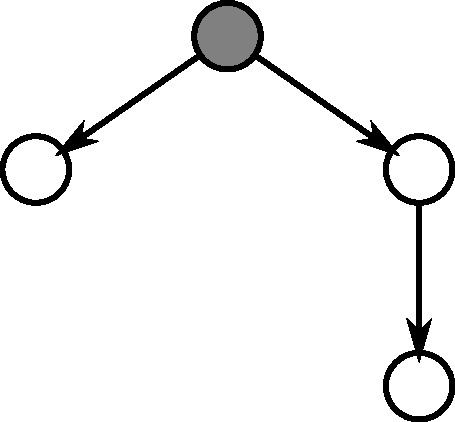
\includegraphics[scale=0.2]{Graphen/baume2.pdf} 
			\vfill
		\end{minipage}
		\begin{minipage}{0.2\linewidth}
			\vspace*{\fill}
			\centering
			\includegraphics[scale=0.2]{Graphen/baume3.pdf} 
			\vfill
		\end{minipage}
		\begin{minipage}{0.2\linewidth}
			\vspace*{\fill}
			\centering
			\includegraphics[scale=0.2]{Graphen/baume4.pdf} 
			\vfill
		\end{minipage}
	\end{center} \pause
	\textit{Zeichnen Sie alle möglichen ungerichteten Bäume mit genau fünf Knoten, von denen keine zwei isomorph sind.} \pause
	\begin{center}
		\begin{minipage}{0.2\linewidth}
			\vspace*{\fill}
			\centering
			\includegraphics[scale=0.2]{Graphen/baume5.pdf} 
			\vfill
		\end{minipage}
		\begin{minipage}{0.25\linewidth}
			\vspace*{\fill}
			\centering
			\includegraphics[scale=0.2]{Graphen/baume6.pdf} 
			\vfill
		\end{minipage}
		\begin{minipage}{0.35\linewidth}
			\vspace*{\fill}
			\centering
			\includegraphics[scale=0.2]{Graphen/baume7.pdf} 
			\vfill
		\end{minipage}
	\end{center}
\end{frame}


\begin{frame}{Aufgabe: Bäume (WS 2010) \stars{1}}
	Sei $T_1 = (V_1 , E_1 )$ ein gerichteter Baum mit Wurzel $r_1$, $T_2 = (V_2 , E_2 )$ ein gerichteter Baum mit Wurzel $r_2$, und es gelte $V_1 \cap V_2 = \{\}$. Sei $r \not\in V_1 \cup V_2$. \\
Zeigen Sie: $$T_1 \circ_r T_2 = (V_1 \cup V_2 \cup {r}, E_1 \cup E_2 \cup \{(r, r_1 ), (r, r_2 )\})$$ ist ein gerichteter Baum mit Wurzel $r$.
\end{frame}

\begin{frame}{Lösung}
	\textit{Zeigen Sie: $$T_1 \circ_r T_2 = (V_1 \cup V_2 \cup {r}, E_1 \cup E_2 \cup \{(r, r_1 ), (r, r_2 )\})$$ ist ein gerichteter Baum mit Wurzel $r$.} \\[2em] \pause
	Zwei Dinge sind zu zeigen:
	\begin{itemize}[<+->]
		\item Zu jedem $v \in V_1 \cup V_2 \cup {r}$ gibt es einen Pfad von $r$ aus
		\item Dieser Pfad ist eindeutig.
	\end{itemize}
\end{frame}

\begin{frame}{Lösung}
	\textit{Wir zeigen zuerst, dass es von $r$ zu jedem Knoten $v \in V_1 \cup V_2 \cup \{r\}$ einen Pfad
gibt.} \\[2em]
	\pause
	\begin{itemize}[<+->]
		\item Es gibt offensichtlich einen Pfad (der Länge 0) von $r$ nach $r$.
		\item Sei $v \in V_1$. Dann gibt es nach Definition einen Pfad von $r_1$ nach $v$ über den Baum $T_1$ und dessen Kanten $E_1$. Da in $T_1 \circ_r T_2$ auch der Pfad $r$ nach $r_1$ liegt, gibt es also einen Pfad von $r$ nach $v$ in $T_1 \circ_r T_2$.
		\item Analog zu $v \in V_2$.
	\end{itemize}
	\visible<5>{Somit gibt es für alle Knoten $v \in V_1 \cup V_2 \cup \{r\}$ einen Pfad von $r$ nach $v$.}
\end{frame}

\begin{frame}{Lösung}
	\textit{Wir zeigen nun noch, dass es für keinen Knoten zwei verschiedenen Pfade von r nach v gibt.} \\[2em]\pause
	Für $v = r$ gibt es offensichtlich keine zwei verschiedenen Pfade. \pause \\ Sei also exemplarisch $v \in V_1$. Da $V_1 \cap V_2 = \{\}$, sind von $r_2$ nur Elemente aus $V_2$ zu erreichen. Somit muss ein Pfad von $r$ nach $v$ über $r_1$ gehen (weil von $r_2$ kein Pfad zurück führt). \pause Da $T_1$ aber ein Baum ist, ist der Pfad von $r_1$ nach $v$ eindeutig. Der Pfad von $r$ nach $r_1$ ebenso. \pause Also ist der Pfad von $r$ nach $v$ auch eindeutig. Analog zu $v \in V_2$.
\end{frame}

% Pufferaufgabe
\begin{frame}{Aufgabe (WS 2009) \stars{4}}
	Eine Zahl $n$ ist genau dann eine Primzahl, wenn sie eine positive ganze Zahl ist und genau zwei Teiler hat, nämlich 1 und n. Insbesondere ist 1 keine Primzahl. \\
	Für $n \in \N^+$ sei der Graph $G_n = (V_n , E_n )$ gegeben durch
	$$V_n =\{m \in \N^+ \ | \ m \text{ teilt } n\}$$
	$$E_n =\{(k, m) \in V_n \times V_n \ | \ k \text{ teilt } m \text{ und } m/k  \text{ ist eine Primzahl} \}$$
	\begin{itemize}
		\item Zeichnen Sie $G_{12}$ , $G_{16}$ und $G_{30}$.
		\item Zeigen Sie: $$\forall \ n, m \in \N^+: n \text{ teilt } m \implies G_n \text{ ist Teilgraph von } G_m$$.
	\end{itemize}
\end{frame}

\begin{frame}{Lösung}
	$$V_n =\{m \in \N^+ \ | \ m \text{ teilt } n\}$$
	$$E_n =\{(k, m) \in V_n \times V_n \ | \ k \text{ teilt } m \text{ und } m/k  \text{ ist eine Primzahl} \}$$
	\textit{Zeichnen Sie $G_{12}$ , $G_{16}$ und $G_{30}$.} \\[1,5em]
	
	\visible<2>{
		\begin{center}
			\begin{minipage}{0.2\linewidth}
				\vspace*{\fill}
				\centering
				\includegraphics[scale=0.2]{Graphen/Primzahlen1.pdf} 
				\vfill
			\end{minipage}
			\begin{minipage}{0.5\linewidth}
				\vspace*{\fill}
				\centering
				\includegraphics[scale=0.2]{Graphen/Primzahlen2.pdf} 
				\vfill
			\end{minipage}
			\begin{minipage}{0.2\linewidth}
				\vspace*{\fill}
				\centering
				\includegraphics[scale=0.2]{Graphen/Primzahlen3.pdf} 
				\vfill
			\end{minipage}
		\end{center}	
	}
\end{frame}	

\begin{frame}{Lösung}
	\only<1|handout:1>{$G_{12}$}\only<2|handout:2>{$G_{16}$}\only<3|handout:3>{$G_{30}$}
	\vspace*{\fill}
	\centering
	\only<1|handout:1>{\includegraphics[scale=0.5]{Graphen/Primzahlen1.pdf}}
	\only<2|handout:2>{\includegraphics[scale=0.5]{Graphen/Primzahlen2.pdf}}
	\only<3|handout:3>{\includegraphics[scale=0.5]{Graphen/Primzahlen3.pdf}}
	\vfill
\end{frame}	

\begin{frame}{Lösung}
	\textit{Zeigen Sie: $$\forall \ n, m \in \N^+: n \text{ teilt } m \implies G_n \text{ ist Teilgraph von } G_m$$}\\[2em] \pause
	Gelte also $n$ teilt $m$. Zu zeigen sind zwei Dinge:
	\begin{itemize}
		\item $V_n \subseteq V_m$
		\item $E_n \subseteq E_m \cap V_n \times V_n$
	\end{itemize}
	
\end{frame}

\begin{frame}{Lösung}
	\textit{Zuerst $V_n \subseteq V_m$.} \\[1em] \pause
	Sei $v \in V_n$ beliebig. Nach Definition gilt: $v$ teilt $n$. Da $n$ aber $m$ teilt, muss $v$ auch $m$ teilen, liegt also in $V_m$. Also gilt $$V_n \subseteq V_m$$ \pause
	
	\textit{Jetzt $E_n \subseteq E_m \cap V_n \times V_n$.} \\[1em] \pause
	Sei $p$ eine Kante mit $p = (x,y) \in E_n$. Wir haben gezeigt, dass dann $x,y \in V_m$ gilt. Außerdem gilt nach der Definition von $E_n$: $$x \text{ teilt } y \text{ und } y/x \text{ ist eine Primzahl}$$ Somit ist $p$ auch in $E_m$ und es gilt $$E_n \subseteq E_m$$.
\end{frame}